The evaluation is one of the final phases of this project. In this chapter, the team will evaluate different aspects of the projects. 
Here it will be discussed why and how the outcome ended up being what it is today.
This includes how the team worked together, why it gave the result it did, the cooperation with the customer, and how it was working with an overseeing force. 
Furthermore, it will be discussed how the team tackeled challanges during the project, and how the development process worked for the team.
The team has chosen to split the evaluation into three major parts, group evaluation, project evaluation and technology evaluation. 
 
 
This is the final phase of this project, the evaluation. Here it will be discussed why and how the outcome
ended up being what it is today.  
%_______________________________________________________________________________
\section{Group evaluation}
The group evaluation will discuss the social aspects of the project. 
We will discuss the team dynamics, our goals, how we used our role assignment, risk assessment, the supervisor the customer, and other issues regarding group evaluation in general.

\subsection{Team dynamics}
This section will shed light on how the group functioned, the cooperation and how this affected the work.

\paragraph{In general}
The group was randomly put together, and the number of people in this goup was four.
Each person with different a personality and interests. Thus, the team could not expect a perfect atmosphere, but fortunately it was no problem. 
The group has functioned well together and offered each other help when needed. There were no huge conflicts, only constructive discussions. 
The overall teamwork and progression of the project was good.

\paragraph{Communication}
Good communication within a team is important, because it creates a safe and stable working
environment. This issue was addressed early on. It was decided that every decision made in the group should be a result of a democratic process. In this case, that meant making decision by the majority vote.

The communication was done through frequent physical meetings. Mostly because of our
agreement of always sitting in the same work area as much as possible. It turned out to be a good rule for most of the time. When every one was siting togheter it was never difficult to get help from the rest of the group, and it was easy to coordinate the work. One problem was the fact that most of us had completely different schedules, so most often there was a person missing. There were a few situations where the team would have benefited from having the entire group present, but there was nothing the team could have done with the matter though, and fortunately it did not affect us too much. The team solved the problem by using Facebook. If someone had other obligations and they were not able to be precent, then the team, kept in contact though Facebook. This was a suitable solution for us since the team members were available online nearly all the time. This made coordination an easier task, since other members could be consulted at any time. 

There were a few problems with the groups communication. The team were too much dependent on one team member responsible for communication. The team was not always added to get copies of the email written to the supervisor nor the customer. Sometimes the team experioenced confusions regarding if there was a meeting that particular day, or not. It happened that group members met up to meetings that were canceled. Also imporant information came a bit late sometimes, and the and the consequence was that team members did not get enough time to free up their schedule.

Another problem the team experienced with communication was that the different schedules the team had, implicated that the team had to work individually in between workin hours. If a team member worked overtime to free up their schedule a bit, and did not inform the rest of the group that they would not be present at working hours, this affected the motivation for the team members present at working hours. 


In hindsight the team can see a couple of things we could have done better concerning the communication. The team could have done more stand ups. It was difficult to follow up on this when everyone had such different schedules. The team solved this problem by having longer meetings when suggested by a team member, so the team could be able to make the necessary decisions. Still the team could have made more strict rules about stand ups, and this could have made the communication easier.
Another idea that could have helped us communicated better was more communication with the other
groups that took this course. Although the tasks were different, exchanging ideas and experience on group dynamics and processes could have affected us in a positive way. 

Our small group size allowed us to get well known with each other, and this made the communication better.
During the semester the have gotten to know each other pretty well after having spent a lot of hours together. Everyone has grown as individuals by learning from each other, and learning to put aside differences, and focusing on the common goal instead.
In spite of a couple of bumps in the road, the team feel that the issue of communication was handled well.

\paragraph{Work distribution}
The distribution of work in this project has been challenging at times. 
The team had little experience with image processing, and therefore it was hard to be sure about the exact work load, and naturally it was difficult to maintain a balanced workload throughout the project. 
In the beginning the team agreed on what needed to be done, and then group members had to take individual responsibility to perform work on the tasks they were comfortable with. 
In the middle there have been times where it has been hard to maintain a steady work flor because some of the team members were exhange studens, and they wanted to experience Norway as well. 
Sometimes this led to periods of inefficiency. Towards the ending of the project it was a bit stressful. The team planned making the final demo-video in the 5th sprint. Then we had a little trouble with the demo-video, and we had to spend more hours than we first thought, and the team fell a little behind.

\paragraph{Motivation}
All team members where very motivated. Everyone wanted to receive a good grade in this course since the course was very relevant for us. In this course we had to use knowledge from several different courses in previous years. Another motivation was the project task. The fact that the task was interesting increased our motivation and efforts. It was exciting and we had the opportunity to learn something new. Our customer was also a great motivator, and by forcing us to deliver something at the end of each sprint, the team alwasy felt like we had reached a milestone. This way we always felt one step closer at the end of each sprint, and it became very motevating to continue the hard work. 

\subsection{Customer and Project task} 
Our customer, Peder Kongelf, was pleased with the results. During the last customer meeting he informed the team that the project goal was reached, which was to make the audience as a screen at a rock concert, and to do this using image processing.
This project was a proof-of-concept project, and if someone wanted to do further work on our application the only remainin parts would be performance and scalability. 
The team wanted to have a bigger "wow-effect" on the last video demonstration, but we did not have enough resources to conduct this. With the demonstration video it is only possible to see the potential the project has. All in all the customer was satisfied with this result. 

In the evaluation of the customer the team is very impressed with our customer. The project he had given us to work with during this course was extreamly exicting. The team got to work with challenging and new technology, which was really great. The fact that the task was interesting increased our motivation and efforts. He had plenty of experience with working as an consultant, and he was eager to teach us as much as possible. The team also wanted to learn as much as possible from him. He gave us good advice about working together as much as possible, and looking back the team was satisfied with this, otherwise communication challanges could have been much harder. Our customer also helped us with the scrum methodology. He taught the team a lot about everything from epics, user stories, task, estimation, to reviews. The team probably learned more from him than from the lecture about agile development. 

Early on Peder suggested weakly meetings, and he always gave us great feedback, as well as giving an impression of having confidence in the team. Sometimes because he had a great amount of work load the meetings where shortened, but still he was involved and enthusiastic about the project. Of course the team expected some communication problems time to time, like confusion over meeting hours, but but the team addressed these issues and were able to keep ourselves and the customer updated on the progress.

We would not have been able to deliver this end result if not for the great effort and constant feedback from the customer. The experiences and knowledge we got from this project is something we will carry with us for years to come.

\subsection{Supervisor}
Almost every week the group met with the supervisor. In these meetings the progress made by
the group was presented, and the supervisors came with feedback on the report and other
work.It was quite useful to know whether the team needed increase the work speed. 
The supervisors also gave feedback on the content of the report. This was also useful for the team.

Before the meetings the team sent out a meeting invitation to the supervisor.
If there were something in particular the team had questions about, then we sent relevant documents before the meeting, so the supervisor could get a chance to look at it before the meetings.

In the beginning the meetings were useful in order to assure that the team were on the right
track. After a while, however, there was less need for a weekly meetings, because the team had a better understanding of what the report should look like.
Maybe a shorter and more informal meeting with the supervisor would have been sufficient, at least for the
middle part of the project 

The communication with the supervisor could have been better time to time. Especially there was a little missunderstanding when the supervisor had to travel to a conferance, and some of the team members showed up to a canceled meeting. This was just little bumps in the road, and most of the time the supervisor was available, and gave us really valuble feedback, especially with the report. 

\subsection{Goals and Milestones} 
"TODO"

\subsection{Challenges}
In this section we will elaborate on some of the challenges that we encounter during the project. Some if the issues were minor, and some where lager. The team will in this section reflect on the challenges we had, and why they occurred, and what we could have done differently.

\paragraph{Time and time estimation}

Throughout the project, time restrictions has been a challange because most of the members in the group have had other projects during the semester. Everyone also had different courses, so suitable working hours for everyone was also a challenge. Agnethe had two different projects in addition to the customer driven project. Milos also had another project that was quite time consuming in the beginning. Jan and Tomas also had another projects besides the customer driven project, and Jan also wanted to take Norwegian classes. All of this made it hard to find working hours. 

Our actual amount of logged work fell a little short of the expected amount of hours. However, the team were able to successfully execute the tasks that we planned.   
The team does not think that the shortage of hours in itself had any significant detrimental effect to the project. The team could probably have done a better job using the planning poker for the estimation, and maybe this could have helped us more. In general, the team think our estimates were within reasonable bounds, but still it could have been better. When looking back the team has definitely gained experience in producing more reasonable estimates.

\paragraph{Language and Cultural Barriers}

Within the team there were three different nationalities, and the natinolalties represented was one Norwegian, one Serbian and two Czechs. Since there were different nationalities within the group, communication had to be done in English. We had to speak english internally in the group, with the supervisor and with the customer. It was a challange to have all communication in english. Solutions and 
technical difficulties is easier to explain in our native language. This caused challanges in decision making. We spend more hours then expected discussing things, because it was hard to express everything correctly, and for everyone to have a clear understanding of the different arguments. Sometimes Jan and Tomas had to switch to Czech. If they had problems expressing their opinions they communicated with smaller comments and questions with each other. Sometimes it was easy to lose focus during discussions when the languange was swiched, but most of the time it was useful.

Since everyone was used to study at different universities, with different cultures and with different ways to do thing. The team sometimes had a different of opinions for solutions. If the team could not reach a decision, it was decided to ask the supervisor or customer to get additional information, and then try to make a new decision. Very often this helped to shed new light on the situation.  For the most of the time language and cultural differences was not a problem, and we were all excited to learn from, and teach each other. 

\subsection{Role assignment}
As mentioned earlier the role assignment was adapted a bit, so it could fit our project better. Also the roles that was assigned to each group member was more of a guideline, rather than a binding responsibility. This was mainly because or some of the team members this was their first scrum project, and some of the roles required more experience and knowledge than the respective group member had. To solve this problem we often devided the roles over several group members depending on the context and situation. Working with the architecture for example often required more than one person responsible. 

When we look back at the role assignment we realize that since we were working with many technologies all of us were unfamiliar in the beginning, it might have been a good idea to make each of the role's responsibility more clear, and maybe spend some time enforcing these responsibilities in the early stages of the project. Also, we should have spent more time finding researching which roles we needed, because some of the roles we assigned we did not use. Even though we decided to embrace this as an equal development team, the roles might have been useful for us. 

These are the roles we assigned, and this is how we evaluated them.

\paragraph{Project Leader}
The project leader was supposed to be responsible for the project progress, and delegate tasks to the other team members. This did not work, because the tasks was prioritized by the customer. If one task was done, the team member had picked the task with the highest priority. All of the team members took responsibility for the progress of the project, and tried to make sure that is went according to the plan. The description also claimed that the Project Leader had final call in arguments, but no group member felt the need to have one person in charge. We chose to embrace this as an equal development team, and that worked well for us.

\paragraph{System Architect}
The system architect was responsible for checking and analyzing all the layers in the product, but this was also something not only one person took responsibility for. 

\paragraph{Scrum Master}
Also the Scrum Master role was assigned to one person originally, but every team member took responsibility for following up on this. It became natural for all of the team members to suggest to have stand ups when we had working hours. It was not always easy too keep track of what the other team members where working on, and this problem occurred since the team were not able to have working hours everyday. The reason for this was that the team members had other courses with projects as well, and therefore we were not able to meet up every day. Having the whole team responsible for scrum methodology worked well for us.

\paragraph{Communication Responsible}
This role is the only that was used throughout the whole project was the customer and supervisor contact responsible. Although this was not a high workload, it was easier for both the customer and supervisor to have one person to communicate with when they had questions.  

\paragraph{QA Responsible}
The QA was responsible for the quality of all documents and also the end product, but the whole team felt responsible for delivering a product with good quality. The QA is also supposed to help with determening is stories and acceptance criteria are well defined, and if they satisfy the requirements.The problem we had with this was that it is hard to conduct if the team member responsible is not that experienced with the scrum methodology. A QA is also responsible for organizing testing, and this includes that unit tests are well written, provide developers with high level test cases for the stories, and performing explorotory tesing on early builds, but in our project we did not focus on the testing part. 

\paragraph{Documentation Responsible}
Also this was a role that every team emmber took responsibility for. It was good to have one person resonsible to set up a good structure in the beginning, but when we started writing more of the conents everyone participated where they could. 

\subsection{Risk evaluation}
In this sections the risks from the risk table in "TODO" section will be evaluated. Among these risks the team only experienced a few of them in some extent.

\paragraph{Sickness/Absence}
Since some of the team members where exchange studens they wanted to travel and experience Norway. The fact that the exchange students wanted to experience Norways was very understandable, but naturally it lead to some abcsence at times. When this happened the team members worked extra hard for this not to affect the procjet. 

\paragraph{Coding problems}
To some extent the team experienced some coding problems, but the team figured it out. At the end it was possible for us to reach the project goals. 

\paragraph{Testing problems}
This problem did not occur, since the customer told us not to focus on the testing part.We tested the application manually, but it was not impemented tests. Therefore testing problems did not occur. What did occur was when er tested the application manually the team sometimes discovered bugs, which needed to be fixed. 
\paragraph{Changing requirements} 
The team did not experience problems with requirements changing. The the communication with the customer was really good, and because of this the problem was avoided.

\paragraph{Dead end with technologies}
While doing research for existing solutions the team experienced difficulties. The team could not find a good existing solution. Luckily the team found OpenCV, and by using this it was possible for us to finish our project. 

\paragraph{Unrealistic time estimation}
It was not easy to estimate all of the user stories. Sometimes the team underestimated and other times the team overestimated. Towards the ending of the project it was a bit stressful, but mostly this did not affect our project.

\paragraph{Customer too ambitious}
The team did not experience that the customer was too ambitious. The reason for this was because the communication with the customer through out the project was very good. The team and the customer had good sprint reviews, and planned the next sprint togheter.

\paragraph{Hardware problems}
The team had some hardware problems. For this project the team were dependent on borowing phones, to be able to test the system. It was not easy to borow phones from a lager amount of friends at the same time. The hardware problem was that the team did not have enough resourses. Luckily the team was able to borow phones two times, the first time the team experienced some troubles with the school network. Phones connectiong to different subnets at NTNU made it difficult for us to test the devices. To solve this problem we needed a router, but it was hard to borow one. The problem was solved by shooting the final demo-video at one of the team members apartment.  


16.2. WORK DISTRIBUTION CHAPTER 16. PROJECT EVALUATION
more than others, especially early in the project phase. An attempt has been done by the project manager to gain complete overview of all assigned tasks, but this has not been successful.
To overcome this problem, we divided the group in two teams and started delegating work to each other rather than leaving the delegation to the project manager. An effort was also made to improve the communication among the group members. This was done to make sure that everyone had an overview of currently assigned work.
R6. Misunderstanding between group members
We have not had any major misunderstandings, however, we did some duplicated work in sprint 2. This would have been avoided if we had communicated better internally.
R9. Unable to work efficiently with the C-language
We started experimenting with the C programming language in order to gain some expe- rience. However, we decided that the C-language was inefficient for us, we had to write a lot of code to perform the simplest task, for instance split a string. Therefore, we changed programming languages for Python.
R10. Unable to work efficiently with Scrum
We had a little workshop for the group in order to familiarize ourselves with Scrum. Only parts of Scrum were implemented in the project, such as sprints, backlog items and daily meetings. The two first sprints were ineffective due to our lack of experience with Scrum. The degree of effectiveness was improved in sprints 3 and 4.
R14. Lack of needed support
There have been some issues where the support from Freescale Semiconductor has not been given when needed. Freescale Semiconductor provided us with sensors at the begin- ning of the project, but they were all delivered without any form of documentation. A workshop with representatives from Freescale Semiconductor was planned, but the event was not held until several weeks of the project was passed. This caused a delay and some ineffective weeks before data gathering and development of algorithms could start.
R15. Uncertainty on customer requirement
There has been some uncertainties regarding the customer requirements, especially early in the project. The customer was eager to extend the scope of the project during the initial project phase, but we felt this was wrong due to our lack of experience.
R16. Hardware gets damaged during gathering of fall data
During the test period, we managed to damage one of the sensors, although the sensor was well protected. The damaged sensor was sent to Freescale Semiconductor for repair, but was never returned due to low availability of qualified lab technicians.
%_______________________________________________________________________________
\section{Project Evaluation}
This section will start with an evaluation of the planning phase and our preliminary studies.  
Then the team will look at our use of the scrum methodology, and how the team had to modify it for our project, before moving on to a discussion of our conduction of meetings. 
\subsection{Planning}
In the following section the team will look at the project plan, evaluate how good it was and to
what degree it was followed through the project.

\subsection{Preliminary Studies}
"TODO"

\subsection{Scrum}
The scrum development methodology was chosen early on even though some of the team members were not too familiar with this sort of development process.
Still there were many good reasons why we chose Scrum to be our development method.
One of the reasons was the highly volatile nature of requirements.
It is also easier to monitor the progress the group was making, and producing working code early was some of them. Also the fact that the team would most likely be using agile methods in most future projects. 
This was also the methodology the customer wanted us to use. 

Using Scrum was difficult at first as only some of us had any previous experience. 
In addition, the project scope was not properly set at the beginning, which made building the product backlog difficult. 
The team did not follow the Scrum convention for user stories as an example. 
All of the stories had to be changed later to make them more consistent. 
The backlog also contained stories for writing the report and attending meetings.
The team decided to add this to report anyways, because it showed very clearly how the had carried out the project from the start til the end. 

Even though the team tried to adapt scrum to our project another negative experience using this methodology was the stand ups. The team should probably have done more stand ups, but the problem was different scheduals. As a student there are several courses to take into account, and this made daily stand ups difficult to follow through. Therefore Scrum would possibly have worked better if we had worked more as a unit with set routines and more strict working hours.

The positive experience was that the concepts of sprints, everything from planning to retrospective was well conducted. The team held a demo presentation for both the customer and the advisor at the end of every sprint, and this helped us keeping them updated on our progress, and opened for feedback. Based on this feedback we could make the necessary changes before it was too late.

Even though the team have had some difficulties with Scrum, the team are glad for using this methodology. Scrum made it simple to implement changes in the project, and continuously produce results that could  be discussed with the customer. It would have been challenging to complete the project using the waterfall model since it was imporant to start the implementation early. To produce all documentation before starting the implementation would also have been difficult. 

In the end we were able to deliver a product that we and the customer were very happy with, which in hindsight can make us say that we were right to choose Scrum.
%_______________________________________________________________________________
\subsection{Course feedback}
In this section there will be an evaluation of the Customer driven development course. The team will evaluate the lectures given in this course, and evaluate the course in general.
The course in general, the project task and the lectures will be evaluated.

\subsubsection{The lectures}
In this section the team will evaluate the different lectures that were held in this course.

\paragraph{Course in group dynamics}
This course focused on making the participants aware of that everyone is different, and handles things differently. Another important focus was the awareness of collaboration. The course made the team more aware of that working together will get us further. It also made the team aware that the other group members can help with refelction during a decision making. The course also forced us to discuss the groups different goals, and the different expectations. 

This course was one of the more useful lectures, since it improved the awareness of people's differences
and that their way of behaving is different, and that forced the team to discuss how to make decisions and solve conflicts if they occured. To give some criticism, it can be mentioned that this course should have been earlier in the semester.

\paragraph{Presentation in agile software development and estimation techniques}
This lecture focused mainly on Scrum methodolody, but it also compared agile software development to other methodologies. This lecture was helpful for the team because i was decided to work in Scrum. Since only one team member had used this methodolody before, it was helpful for the team to learn more about the basics. 

\paragraph{Seminar in technical writing}
This lecture was useful since it gave the team a understanding of how a technical report should be written. The only critique is that some of the feedback the team got was not consistent with the feedback given by the supervisor.

\paragraph{Course in presentation technique}
During this lectures the team had some trouble making the final demonstration, which meant the team had to prioritize fo finish the final demonstration video, and could not attend this course.

\subsubsection{Final comments}

All in all this has proven to be a very valuable course. It has given the team a proper insight into the how’s and why’s of the whole software development process. Everything from the very start to the very end of a large project. The team have learned how to plan and estimate, research, learned more about implementation, and of course working together as a team. 

It has been a welcome change to work with a real customer and learning more about working as an consultant.It has been a huge motivation for the team to work with a real customer, because the team really wanted to deliver something the customer would be pleased with. There is a fine line between upholding the initial requirements, and tuning them with the customers changes throughout a project. The team feel that we have upheld our stronghold, but at the same time opened a few doors to
make the customer happy without burdening ourselves too much. We can with this information
conclude that it has been a successfull project.
%_______________________________________________________________________________
\section{Technologies and tools evaluation}
In this section you can read about main used technologies and tools during developing.
Emphasis is placed on problems encountered during using these tools and technologies.

\subsection{Android}

\subsection{OpenCV}
OpenCV is an open source computer vision library briefly described in section \ref{subsec:image_processing_library}.
It is a very useful library, which saved the team a lot of time instead of implementing image processing parts themselves
 -- whole light detection module was just enhanced demonstration example of OpenCV functionality.

On the other hand, some problems with this library occurred.
OpenCV Java API is a relatively new and therefore some implementation is missing.
One example of this was described in section \ref{sec:sprint3_implementation}.
This raised a lot of problems, which resulted into discarding of user story.

OpenCV Java API can be therefore counted as a immature product but with a high potential in future, provided OpenCV developers will focus more on this API.
At this moment, new release 2.4.7 if OpenCV is 44 days late according to the plan\footnote{\url{http://code.opencv.org/projects/opencv/roadmap}} with still 32 opened bugs or new features.

\subsection{Git}
The team adopted Git as its version control system since early phase as described in section \ref{subsec:git}.
Most of the members had experience with some other VCS such as Subversion and therefore the idea of versioning was not new.
On the other hand, three of four members of the team had no experience with Git itself.

Even though Git is a powerful tool with a lot of features, the main reason of using was to share code.
Since development was rather linear, branching was used rarely.
On the other hand, support of releases was used quite often \footnote{\url{https://github.com/dohnto/DigitalLighter/releases}}.
This was very comfortable for creating a final report, when the team could easily see exactly what features were included in each prototype and also it was possible to se the GUI of product in particular phase.

Of course, troubles during merging occurred.
Since merging conflicts can be sometimes demanding and usually requires a deep knowledge about merging code, sometimes it was impossible for one person to solve it.
These conflicts were in most cases solved by discussion with all interested members.

After all the experience with Git is rather positive. 
It is always good to be able to work with tools, that a lot of companies use in real development.


\subsection{Target Process}
Target Process is a collaborative project management tool described in section \ref{subsec:targetProcessToolDescription}.
This tool was chosen after two another tools were tried.
It is very complex tool for large teams and it provides many different views on project (called boards) and also offers to personalize these views.

This tool was used mainly for a collaboration with customer. 
Before sprint planning, user stories for next sprint were prepared and inserted into Target Process.
Customer could easily prioritize these stories by dragging and dropping.
He could also see spend hours on particular story and also the progress bar depicting progress of this story.

Sometimes, due to lack of a discipline, the spend hours and finished stories and tasks were not filled in time and therefore the retrospective cannot be that precise.
Anyway, Target Process was very mature and useful tool for customer communication with much more features that was for this project necessary.


\subsection{TestFlight}
TestFlight service, described in section \ref{subsec:testflight}, was adopted because of customer proposal.
The service was used in early phases of development for customer comfort when testing the product.

Since the beginning of implementation, some non-reproducible errors occurred in client application.
After some testing, the team suspected TestFlight of those problems.
TestFlight for Android is relatively new service \footnote{\url{http://blog.testflightapp.com/post/49971420302/android}} and there it was decided to discard it from the implementation.
After some time, the team has discovered, that the issues were caused by Android system itself 
%___________-_______________________________________
(REF NEEDED)
%__________________________________________________-
, but the TestFlight was never used again, because the demonstration for customer were performed in form of videos.
 
Therefore it is difficult to evaluate tool, that has been used only for a short period of time.

\subsection{Technical issues}
During testing light detection module, problem situation\footnote{Tested with Samsumg Galaxy S3 and Samsung Galaxy S2.} with mobile devices camera was encountered.
In dark, if a tracked object (mobile phone lighting with single color) or camera itself is moving, everything is working as expected.
But if both object and camera are static, after some time, the camera starts to adjust the colors.
You can see that situation in Figure \ref{fig:screen_colors_in_enviroments}.
This is probably caused by exposure settings, and further research concerning that topic would have to be done.
\begin{figure}[h]
        \centering
        \begin{subfigure}[b]{0.4\textwidth}
                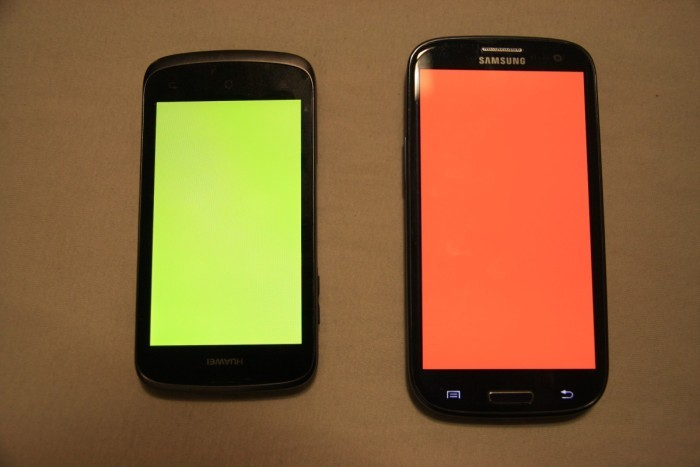
\includegraphics[width=\textwidth]{evaluation/IMG_7029.JPG}
                \caption{Colors of screens in light environment}
                \label{fig:tiger}
        \end{subfigure}
        ~ %add desired spacing between images, e. g. ~, \quad, \qquad etc.
          %(or a blank line to force the subfigure onto a new line)
        \begin{subfigure}[b]{0.4\textwidth}
                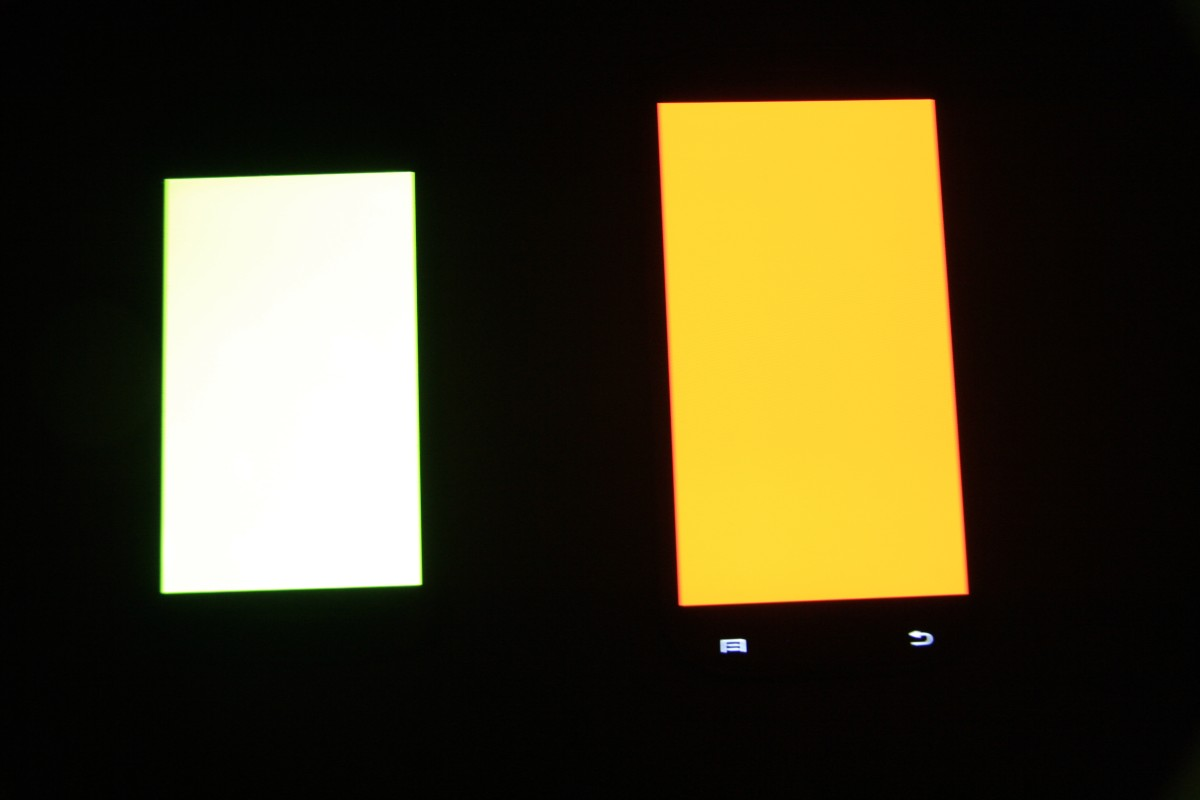
\includegraphics[width=\textwidth]{evaluation/IMG_7032.JPG}
                \caption{Colors of screens in dark environment}
                \label{fig:mouse}
        \end{subfigure}
        \caption{Colors of screens in different light environments}\label{fig:screen_colors_in_enviroments}
\end{figure}
By empirical research there were established colors (e. g. blue and white) which are least affected by this behavior.
